\section{Results}

\subsubsection{Results - Linear Model}
Subsubsection text here.
\begin{figure}[t]
    \centering
    \begin{minipage}[b]{0.45\columnwidth}
        \centering
        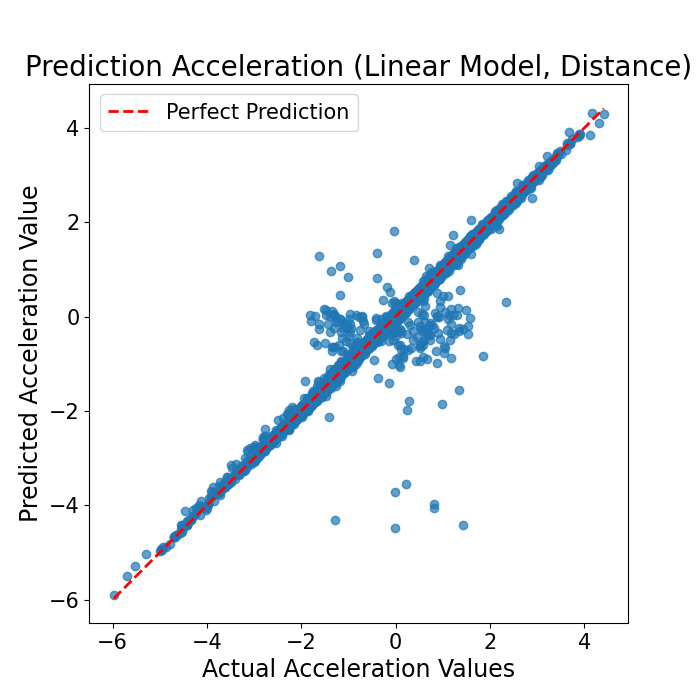
\includegraphics[width=\columnwidth]{images/figures/Prediction Acceleration (Linear Model, Distance).png}
        \caption{Caption for Figure 1}
        \label{fig:minipage3}
    \end{minipage}
    \hfill
    \begin{minipage}[b]{0.45\columnwidth}
        \centering
        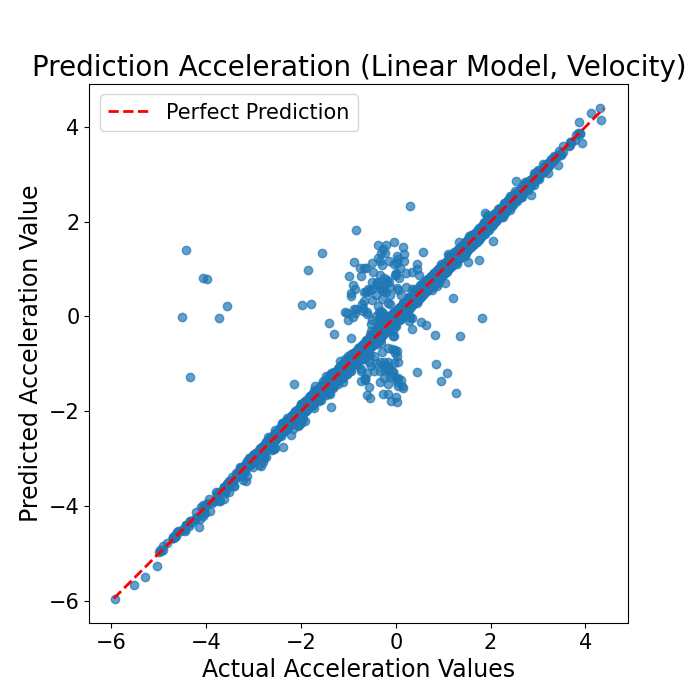
\includegraphics[width=\columnwidth]{images/figures/Prediction Acceleration (Linear Model, Velocity).png}
        \caption{Caption for Figure 2}
        \label{fig:minipage4}
    \end{minipage}
    \caption{Caption for the entire figure}
    \label{fig:combined_figure_2}
\end{figure}


\begin{figure}[t]
    \centering
    \begin{minipage}[b]{0.45\columnwidth}
        \centering
        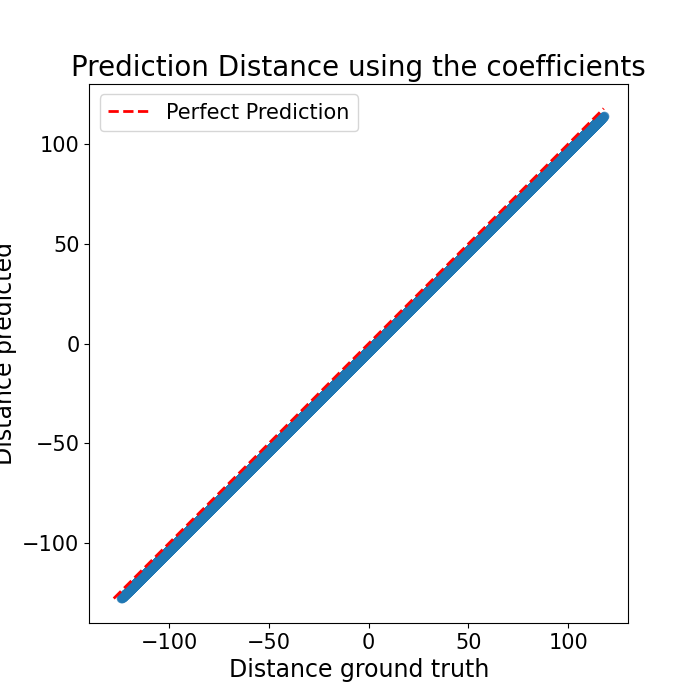
\includegraphics[width=\columnwidth]{images/figures/Prediction Distance using the coefficients.png}
        \caption{Caption for Figure 1}
        \label{fig:minipage3}
    \end{minipage}
    \hfill
    \begin{minipage}[b]{0.45\columnwidth}
        \centering
        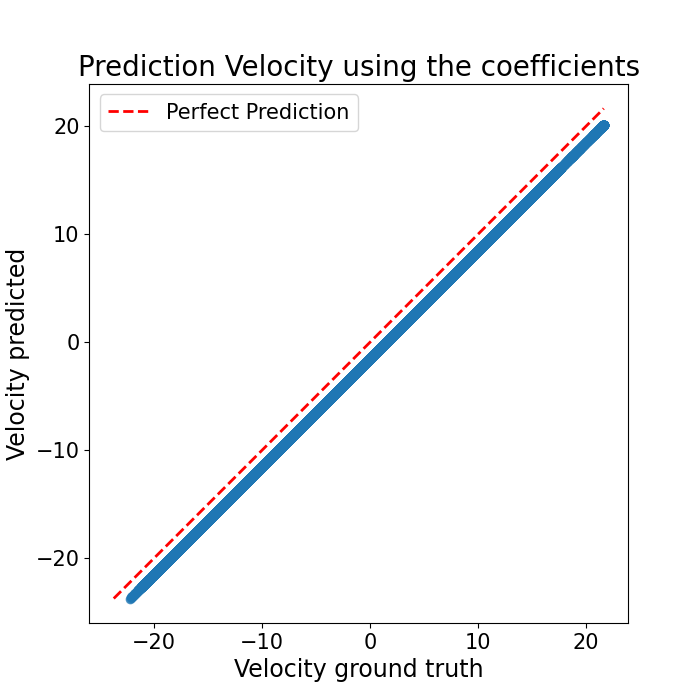
\includegraphics[width=\columnwidth]{images/figures/Prediction Velocity using the coefficients.png}
        \caption{Caption for Figure 2}
        \label{fig:minipage4}
    \end{minipage}
    \caption{Caption for the entire figure}
    \label{fig:combined_figure_2}
\end{figure}


\begin{figure}[t]
    \centering
    \begin{minipage}[b]{0.45\columnwidth}
        \centering
        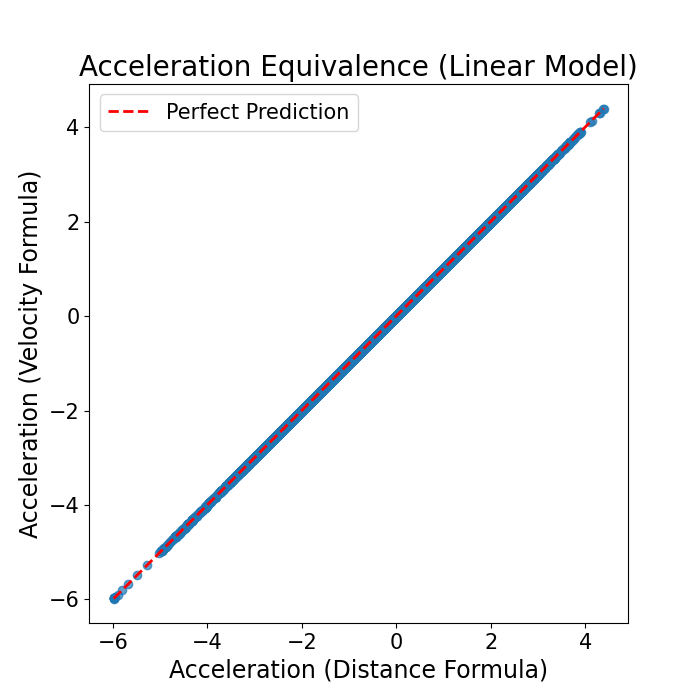
\includegraphics[width=\columnwidth]{images/figures/Acceleration Equivalence (Linear Model).png}
        \caption{Caption for Figure 1}
        \label{fig:minipage3}
    \end{minipage}
    \hfill
    \begin{minipage}[b]{0.45\columnwidth}
        \centering
        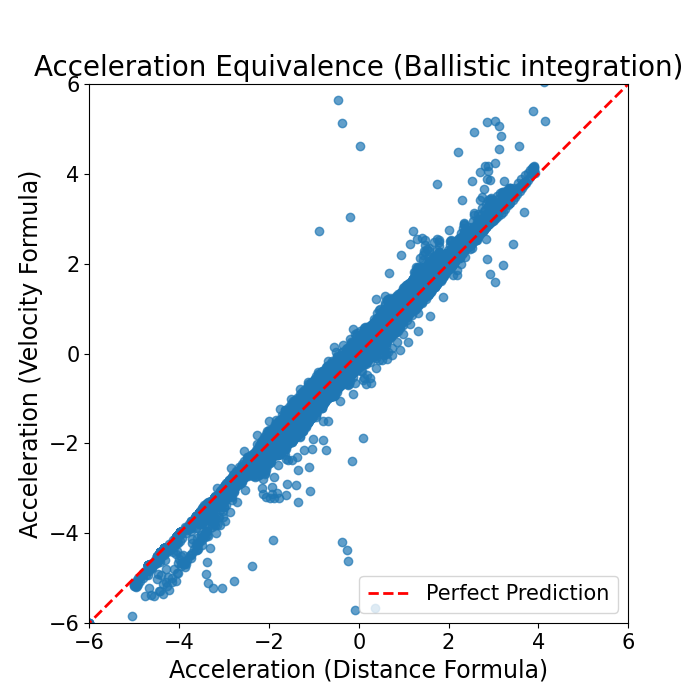
\includegraphics[width=\columnwidth]{images/figures/Acceleration Equivalence (Ballistic integration).png}
        \caption{Caption for Figure 2}
        \label{fig:minipage4}
    \end{minipage}
    \caption{Caption for the entire figure}
    \label{fig:combined_figure_2}
\end{figure}








\subsection{Notable Findings and Observations} 
During the evaluation process, several notable findings were observed. 
Most notably, after rearranging the formula for distance and velocity, a constant error was detected. 
However, increasing the size of NumPy arrays appeared to mitigate this error, indicating a potential 
floating-point precision issue.

\subsection{Future Directions} 
Based on our implementation experience, future research and improvement areas include enhancing the 
precision of NumPy arrays by increasing their size and expanding the dataset to encompass a more extensive
range of scenarios for comprehensive model training and testing.

